\newpage

\section{Rozpraszanie Ramanowskie}
\subsection{Czym jest spektroskopia ramanowska}
Spektroskopia Ramana jest istotną metodą badania widm rotacyjnych i oscylacyjnych cząsteczek. Światło rozpraszane ma inne częstości niż światło padające. Obserwujemy przesunięcie linii zarówno w stronę większych jak i mniejszych częstości, a tym samym większych i mniejszych energii. Kilka cech tej spektroskopii jest niezwykle ważnych. Jedną z nich jest możliwość użycia światła widzialnego do badania widma Ramana. Można lepiej operować takim światłem w warunkach doświadczenia niż światłem podczerwonym lub mikrofalami. Niektóre dwuatomowe cząsteczki jak $\mathbf{H_{2}}$ czy $\mathbf{O_{2}}$ nie posiadają momentu dipolowego i dlatego nie są aktywne w podczerwieni, a ich widma mogą być badane właśnie w widmie Ramana. Zatem np. pod tym względem spektroskopia ramanowska jest dopełnieniem spektroskopii w podczerwieni i odwrotnie. Poza tym spektroskopia ramanowska umożliwia badanie ruchu cząsteczek, które zmieniając swoje położenie, wykonują np. ruchy obrotowe, co z kolei powoduje zmianę ich ukierunkowania względem padającego promieniowania. Objawia się to zmianą polaryzacji w stosunku do światła padającego. Ponadto rozpraszanie Ramana, podobnie jak spektroskopia w podczerwieni, dostarcza informacji o budowie cząsteczki, wiązaniach międzyatomowych, które ją tworzą, a także o ich polaryzowalności. Pozwala to przewidzieć reaktywność chemiczną i przebieg reakcji chemicznych.

Rozproszone fotony co mają określone przesunięcie energetyczne są parametrami do stwierdzenia rodzaju gazu. Aktywne przejścia Ramana, inne niz przejscia w podczerwieni. Wszystkie dwuatomowe gazy homonuklearne są niewidoczne w podczerwieni ($\mathbf{O_{2}}$, $\mathbf{N_{2}}$, $\mathbf{H_{2}}$, $\mathbf{Cl_{2}}$), a w widmie Ramana są widoczne. Dodatkową zaletą spektroskopii ramanowskiej jest to że można identyfikować mieszaninę gazów. Na podstawie tego jest zastosowanie: w wykrywaniu paliwa gazowego dla elektrowni naturalnych lub biogazowych, w których $\mathbf{CH_{4}}$, $\mathbf{CO_{2}}$, $\mathbf{O_{2}}$, $\mathbf{N_{2}}$ i $\mathbf{H_{2}}$ są istotne dla monitorowania, w procesach przemysłowych gdzie ma miejsce $\mathbf{H_{2}O}$, dla tego, że czujniki Ramana są słabo uszkadzane wodą. Pomiar odbywa się na bieżąco. Dalsze zalety czujników gazowych Ramana są w stanie tolerować wysokie stężenia gazu i mieć wysoki zakres dynamiczny, ponieważ nie cierpią z powodu efektów nasycenia. Objętość pomiaru może być bardzo mała w spektroskopii ramanowskiej. Pomiar w mikroreaktorach dla chemii kombinatorycznej. Główną wadą spektroskopii ramanowskiej jest to, że proces rozpraszania jest dość słaby, co oznacza, że jest trudny w uzyskaniu akceptowalnej czułości. Większość spektrometrów ramanowskich są zbudowane do wykrywania ciał stałych lub płynów, gdzie wyższa gęstość materiału znacząco zwiększa sygnał. 

\subsection{Wgląd matematyczny}
Jeżeli światło o natężeniu 
\begin{equation}
	E = E_{m}\cos (2\pi f_{p}t)
\end{equation}
\begin{itemize}
	\item[-]{$E$ - natężenie padającego światła};
	\item[-]{$E_{m}$ - wartość maksymalna natężenia};
	\item[-]{$f_{p}$ - częstotliwość promieniowania padającego}.
\end{itemize}
pada na cząsteczkę, to wystąpi oddziaływanie pomiędzy wektorem $\overrightarrow{E}$, a elektronowymi powłokami atomów tworzących cząsteczkę.
Elektrony w cząsteczkach wykazują polaryzowalność $\alpha$, czyli zdolność przemieszczania
się pod wpływem pola elektrycznego. W wyniku takiego przemieszczenia jest indukowany w cząsteczce moment dipolowy.
\begin{equation}
	p_{i} = \alpha E = E_{m}\cos (2\pi f_{p}t)
\end{equation}
Ponieważ ten moment dipolowy oscyluje z częstotliwością $f_{p}$ następuje emisja promieniowania o tej samej częstotliwości. Ta częstotliwość nosi nazwę 
\textit{rozpraszania Rayleigha}.

Niech cząsteczka wykonuje drgania z częstotliwością $f_{osc}$, to wychylenie z położenia 
równowagi można opisać wzorem:
\begin{equation}
	r - r_{0} = r_{m}\cos (2\pi f_{osc}t)
\end{equation}
\begin{itemize}
	\item[-]{$r_{0}$ - położenie równowagi};
	\item[-]{$r_{m}$ - maksymalne wychylenie};
	\item[-]{$f_{osc}$ - częstotliwość drgań cząsteczki}.
\end{itemize}
Polaryzowalność cząsteczki zmienia się wraz z odległością $r$. Ta wielkość może być
przedstawiona w postaci szeregu potęgowego:
\begin{equation}
	\alpha(r) = \alpha(r_{0}) + \frac{d\alpha}{dr}(r - r_{0}) + 
	\frac{d^{2}\alpha}{dr^{2}}(r - r_{0})^{2} + ... +
	\frac{d^{n}\alpha}{dr^{n}}(r - r_{0})^{n}
\end{equation}
W dalszych przekształceniach nie będziemy uwzględniać wyrazów rzędów wyższych od jednego. 

Uwzględniając wzory (1),(2),(3) możemy przedstawić moment dipolowy cząsteczki w następujący
sposób:
\begin{equation}
	p(t) = \alpha E = 
	\left\{ 
		\alpha(r_{0}) + \frac{d\alpha}{dr}r_{m}\cos (2\pi f_{osc}t) 
	\right\}
	E_{m}\cos (2\pi f_{p}t)
\end{equation}
Możemy przekształcić powyższe równanie po zastosowaniu wzoru na iloczyn cosinusów:
\begin{equation}
	p(t) = \alpha(r_{0})E_{m}\cos (2\pi f_{p}t) + \frac{d\alpha}{dr}E_{m}r_{m}
	\left\{
		\cos (2\pi (f_{p} + f_{osc})t) + \cos (2\pi (f_{p} - f_{osc})t)
	 \right\}
\end{equation}
Ponieważ argumenty funkcji $\cos$ zawierają częstotliwość $f = f_{p} \pm f_{osc}$, w widmie światła
rozproszonego ta częstotliwość będzie obserwowana. Wielkość przesunięcia jest cechą charakterystyczną danej cząsteczki. Lnie widma, które przesunięte w stronę mniejszych energii, są tzw. pasma stokesowskie, a w stronę większych energii – antystokesowskie.
\begin{figure}[H]
	\begin{center}
		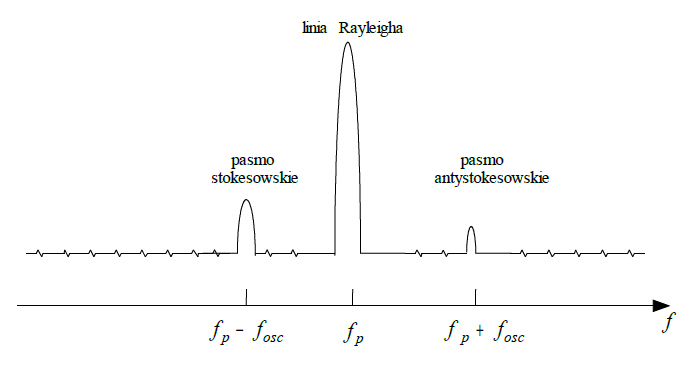
\includegraphics[width=1\linewidth]{Rozpraszanie-Ramanowskie/Schemat-widma-Ramanowskiego.png}
		\caption{Schemat widma ramanowskiego.[4]}
	\end{center}
\end{figure}

\subsection{Rodzaje pasm obserwowanych w widmie Ramana}
W widmie Ramana są obserwowane trzy rodzaje pasm:
\begin{itemize}
	\item[-]{Pasmo Rayleigha};
	\item[-]{Pasmo stokesowskie};
	\item[-]{Pasmo antystokesowskie}.
\end{itemize}

\textbf{Pasmo Rayleigha} - powstające na skutek oddziaływania fotonów padającego promieniowania o częstości $v_{0}$, nie pasujących do poziomów energetycznych cząsteczki. Po oddziaływaniu fotonu z cząsteczką, ostatnia wraca na ten sam poziom energetyczny.

\textbf{Pasmo stokesowskie} - gdy cząsteczka po oddziaływaniu z promieniowaniem przenosi się na wyższy poziom oscylacyjny i rozproszony foton ma energię mniejszą o różnicę energii poziomów oscylacyjnych $hv$.

\textbf{Pasma antystokesowskie} - jeśli przed oddziaływaniem z promieniowaniem molekuła znajdowała się na wzbudzonym poziomie oscylacyjnym, to oddziaływanie przenosi ją na podstawowy poziom oscylacyjny. Energia rozproszonego fotonu jest większa o różnicę energii poziomów oscylacyjnych $hv$. Pasmo antystokesowskie pojawia się w widmie Ramana po przeciwnej stronie co pasmo stokesowskie w stosunku do pasma Rayleigha. Pasmo to ma zwykle niższą intensywność niż pasma stokesowskie.
\begin{figure}[H]
	\begin{center}
		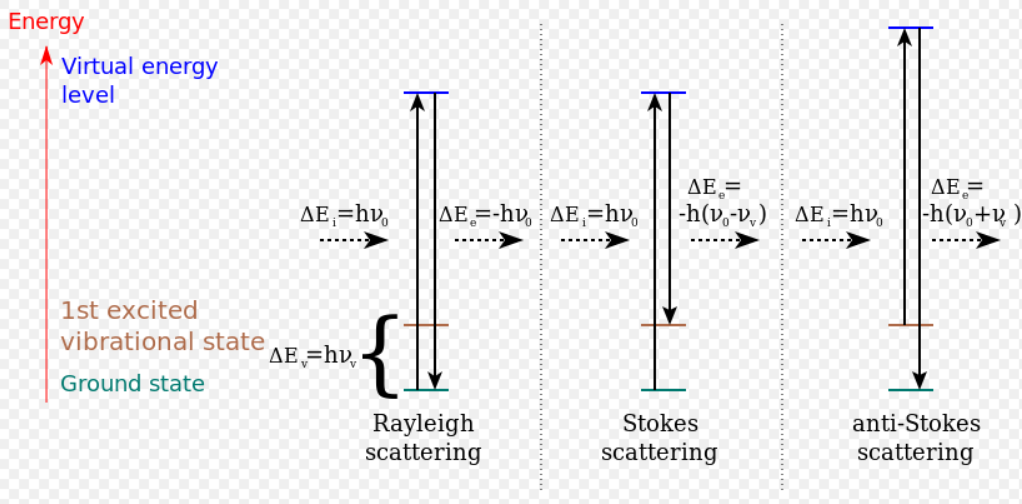
\includegraphics[width=1\linewidth]{Rozpraszanie-Ramanowskie/Raman-Energy.png}
		\caption{Diagram energii przejść w poszczególnych rodzajach rozpraszania.}
	\end{center}
\end{figure}
Widmo antystokesowskie jest mnie intensywne niż widmo stokesowskie. To jest spowodowane tym,
że prawdopodobieństwo oddziaływania fotonu ze wzbudzonym atomem jest dużo mniejsze niż
oddziaływanie z atomem w stanie podstawowym.

\subsection{Czynniki warunkujące zaistnienie zjawiska}
\subsubsection{Idealny dipol}
Przykładem takiego dipola może być układ składający się z spoczynkowego ładunku dodatniego $+Q$ i ładunku ujemnego $-Q$, harmonicznie oscylującego wzdłuż kierunku $\overrightarrow{P}$ z częstotliwością $\omega$.
\begin{equation}
	p = p_{0}\cos(\omega t)
\end{equation}
Problem promieniowania dipola ma istotne znaczenie w teorii układów promieniujących, ponieważ każdy rzeczywisty układ promieniujący (na przykład antena) może być obliczony na podstawie promieniowania dipola. Ponadto wiele pytań dotyczących interakcji promieniowania z materią można wyjaśnić na podstawie klasycznej teorii, biorąc pod uwagę atomy jako układy ładunków, w których elektrony wykonują oscylacje harmoniczne w pobliżu ich pozycji równowagi.

Jeśli fala rozchodzi się w homogenicznym ośrodku izotropowym, to czas przejścia fali do punktów odległych od dipola o odległość $r$ jest taki sam. Dlatego we wszystkich punktach kuli, której środek pokrywa się z dipolem, faza oscylacji jest taka sama, to znaczy w strefie falowej przód fali będzie sferyczny, a w konsekwencji fala emitowana przez dipol jest sferyczną falą.

W każdym punkcie wektory $\overrightarrow{E}$ i $\overrightarrow{H}$ oscylują zgodnie z prawem $\cos(\omega t - kr)$, amplitudy tych wektorów są proporcjonalne do
$\frac{\sin \theta}{r}$ (dla próżni). Czyli one zależą od odległości od $r$ odległości od środka dipola i kąta $\theta$ między kierunkiem momentu dipolowego i kierunkiem promieniowania.
\begin{figure}[H]
	\begin{center}
		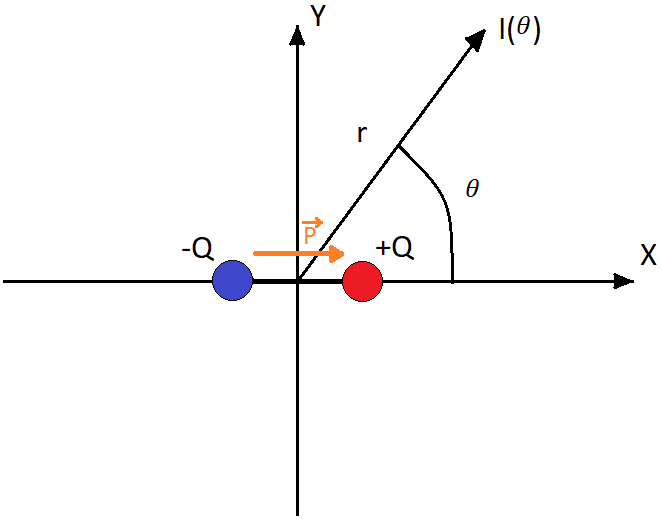
\includegraphics[width=0.6\linewidth]{Rozpraszanie-Ramanowskie/Point-Dipol.png}
		\caption{Drgający dipol, który twarzą dwa ładunki $-Q$ i $+Q$. $I(\theta)$ to jest natężenie promieniowania na odległości $r$ pod kątem $\theta$.}
	\end{center}
\end{figure}
Wynika stąd, że natężenie promieniowania dipolowego wynosi:
\begin{equation}
	I \sim \frac{\sin^{2}\theta}{r^{2}}
\end{equation}
Dla $\theta = \frac{\pi}{2}$ intensywność promieniowania jest maksymalna, a dla 
$\theta = 0$ i $\theta = \pi$ jest minimalna i wynosi $0$. Czyli dipol nie promieniuje wzdłuż kierunku momentu dipolowego.
\subsubsection{Realny dipol}
Warunkiem zaistnienia zjawiska Ramana są zmiany polaryzowalności cząsteczki w trakcie danego drgania. Polaryzowalność jest wielkością, którą można wyrazić za pomocą tensora, który jest układem 9 współczynników:
\begin{equation}
	\alpha = 
	\begin{vmatrix}
	\alpha_{xx} & \alpha_{xy} & \alpha_{xz} \\
	\alpha_{yx} & \alpha_{yy} & \alpha_{yz} \\
	\alpha_{zx} & \alpha_{zy} & \alpha_{zz}
	\end{vmatrix}
\end{equation}
Gdy mówimy np. o indukowanym momencie dipolowym, to pierwszy wskaźnik dwuelementowego indeksu oznacza kierunek momentu dipolowego, a drugi kierunek przyłożonego pola elektrycznego (wektora natężenia pola).

\newpage
\subsection{Przykładowe widma ramanowskie}
Widmo ramanowskie dla materiałów $GaS$ i $Ga_{2}S_{3}$:
\begin{figure}[H]
	\begin{center}
		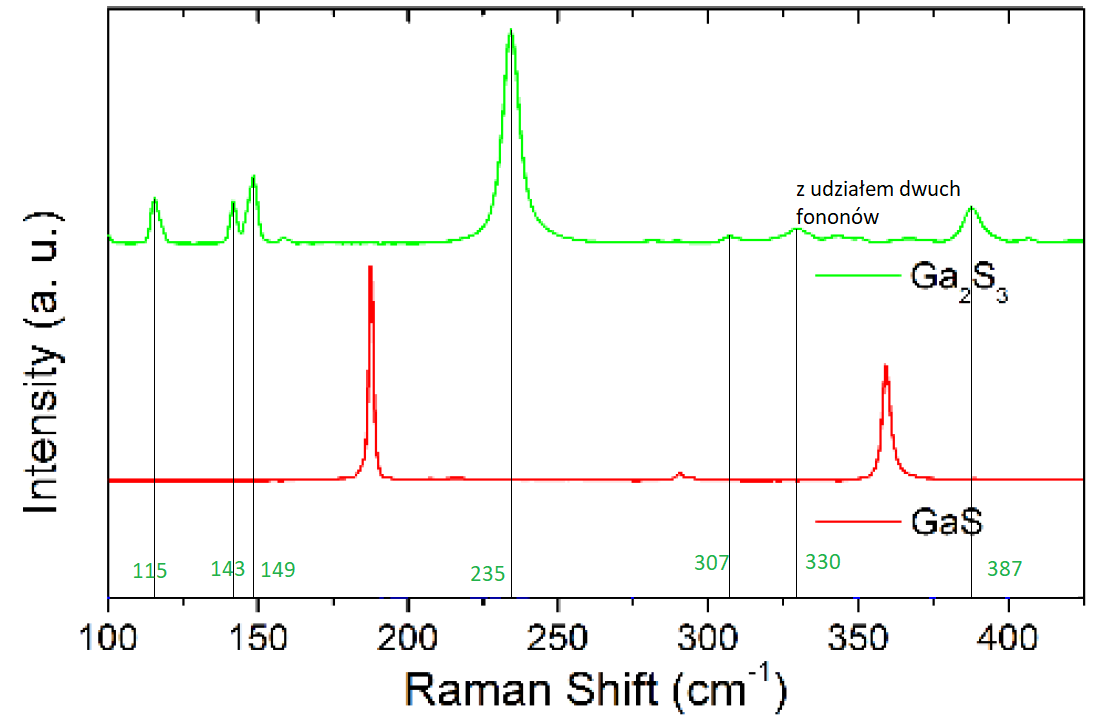
\includegraphics[width=0.8\linewidth]{Rozpraszanie-Ramanowskie/Raman-Shift.png}
		\caption{Widma rozpraszania ramanowskiego dla materiałów $GaS$ i $Ga_{2}S_{3}$[3]}
	\end{center}
\end{figure}
Na powyższym rysunku pokazane tylko pasma stokesowskie, ponieważ tylko tą częścią będę się zajmował w swojej pracy.

Energia fotonu wynosi:
\begin{equation}
	E = h \nu = h \frac{c}{\lambda} = hc \frac{1}{\lambda} 
\end{equation}
\begin{itemize}
	\item[-]{$h$ - stała Plancka};
	\item[-]{$c$ - prędkość światła};
	\item[-]{$\lambda$ - długość fali}.
\end{itemize}
Czyli odwrotność długości jest proporcjonalna do energii:
\begin{equation}
	\lambda^{-1} \sim E
\end{equation}

Zeru na powyższym widmie odpowiada energia światła pobudzającego (lasera) z przesunięciem wynoszącym zero. Czyli przesunięcie w widmie stokesowskim można zapisać w następując sposób:
\begin{equation}
	\frac{1}{\lambda} = \left| \frac{1}{\lambda_{Laser}} - \frac{1}{\lambda_{stok}} \right|
\end{equation}
\begin{itemize}
	\item[-]{$\lambda_{Laser}$ - długość fali promieniowania laserowego};
	\item[-]{$\lambda_{stok}$ - długość fali promieniowania stokesowskiego}
\end{itemize}













